\section{The architecture of a programmable switch}
\label{s:context}

\begin{figure*}
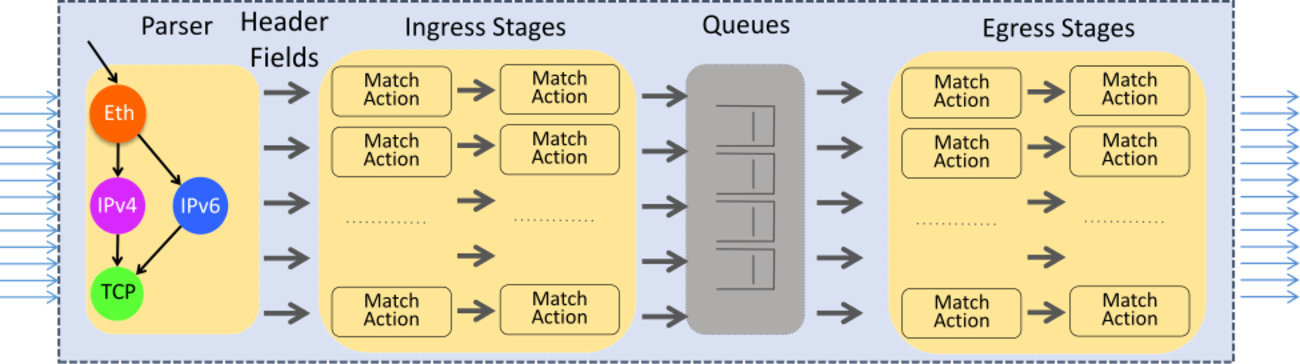
\includegraphics[width=\textwidth]{p4_switch_model.png}
\caption{The RMT architecture}
\end{figure*}

\label{s:architecture}
In this section, we briefly describe the Reconfigurable Match-Action Table
(RMT) architecture~\cite{rmt}, a representative programmable switch
architecture used in our experiments. Other switches with similar programmable
architectures include Intel's FlexPipe~\cite{flexpipe} and Cavium's
Xpliant~\cite{xpliant}.

Figure~\ref{fig:architecture} provides a high-level overview of the RMT
architecture. Packets enter the switch through serial links and are handled by
a programmable parser that turns packets into a bag of header fields. The
ingress and egress pipelines have a number of physical pipeline stages that can
process these header fields using a sequence of match-action tables.

Such tables match on arbitrary header fields and carry out actions in response
to a match.  The actions are built out of simpler action primitives, which
represent simple arithmetic and logic operations on packet fields. To remain
performance competitive with fixed-function switches~\cite{mellanox, broadcom},
each action primitive can modify only one packet field, although several action
primitives can be grouped together into larger actions using a Very-Large
Instruction Word if they can all execute in parallel without violating data
dependencies such as two instructions writing to the same packet field
(Write-After-Write) or an instruction reading from the same packet field that
was written to previously (Read-After-Write).

The RMT architecture also includes a set of atomic stateful operations, i.e.,
operations that allow packets to manipulate persistent state atomically from
one packet to the next.  We summarize these in
Table~\ref{t:stateful_inst}.\footnote{We use the symbols {\tt x} to refer to
stateful variables and {\tt pkt.<>} to refer to a packet field.{\tt
pkt.field} can be substituted for a constant operand in places that are
appropriate.}
\begin{table}
\begin{small}
\begin{tabular}{|c|c|}
\hline
Instruction description & Form \\
\hline
Read and write & \texttt{x = pkt.field;} or \texttt{pkt.field = x;} \\
\hline
Read, modify, and write & \texttt{x = x + pkt.field;} \\
\hline
Conditional execution & \texttt{x = pkt.predicate ? pkt.field : x;} \\
\hline
\end{tabular}
\end{small}
\caption{Atomic stateful instructions in the RMT architecture}
\label{t:stateful_inst}
\end{table}
%\item Packed operations on pairs of stateful variables: \texttt{ (x, y) = (x + y, x - y);}
%\item Multiply and accumulate a stateful variable: \texttt{ x = x * pkt.field + pkt.field2; }

RMT is a shared-nothing architecture: state variables are local to a particular
stage in the ingress or egress pipeline and cannot be shared across pipeline
stages or pipelines. The RMT pipeline allows a stage to communicate state
information to a successor stage downstream by writing state into a packet
field. To let a stage communicate state information to a predecessor stage
upstream, the RMT architecture allows packets to be cloned and recirculated
back into a pipeline.

This way, a state variable can be read in stage x, written downstream in stage
y, and then a cloned packet to stage x could update the state variable in x.
However, recirculation has a cost: recirculated packets consume pipeline
capacity by taking away capacity from new data packets. Further, recirculation
latency can be large: several hundred packets might pass through the pipeline
before the recirculated packet update state in stage x.
